\documentclass[../main]{subfiles}
\begin{document}
    \section{Dinámica Hamiltoniana}
Considerando un sistema con $n$ coordenadas generalizadas($n$ grados de libertad) ($q_1, \cdots, q_n$) y lagrangiano $L(q_1, \cdots, q_n, \dot{q}_1, \cdots, \dot{q}_n, t)$. Entonces tiene $n$ ecuaciones diferenciales ordinarias de 2do orden en el tiempo, denominados ecuaciones de Lagrange 
\begin{equation}
    \dv{}{t}\left(\pdv{L}{\dot{q}_i}\right)-\pdv{L}{q_i}=0,\quad i=1, \cdots, n.
\end{equation}

La teoria Hamiltoniana fue desarrollada por Hamilton en el siglo XIX. Está basada en la sustitución de las $n$ ecuaciones de movimiento dadas por la ecuación de Lagrange, por un conjunto duplicado ($2n$) de ecuaciones diferenciales ordinarias de primer orden en el tiempo, este método consiste en la reducción del orden en el tiempo de las ecuaciones diferenciales ordinarias.

\subsection{Formulación Hamiltoniana}
Se introducen $2n$ coordenadas:
\begin{equation}
    (q_1, \cdots, q_n, p_1, \cdots, p_n)
\end{equation}

Se construye una función 
\begin{equation}
    H(q_1, \cdots, q_n, p_1, \cdots, p_n, t)
\end{equation}

Las ecuaciones de movimiento son ahora $2n$ ecuaciones diferenciales ordinarias de primer orden denominadas \textbf{ecuaciones de Hamilton}.

\subsubsection{Reduciendo el orden}
Sea $\dot{q}_i \rightarrow S_i$, entonces 
\begin{equation}
    L(q, \dot{q}, t) \rightarrow L(q, S, t)
\end{equation}
La ecuación de Lagrange será 
\begin{equation}
    \dv{}{t}\left(\pdv{L}{\dot{q}_i}\right)-\pdv{L}{q_i}=0 \ \rightarrow \ \dv{}{t}\left(\pdv{L}{S_i}\right)-\pdv{L}{q_i}=0
\end{equation}
en esta teoría de Hamilton $p$ representa los momentos canónicos conjugados.
\subsubsection{Momentos Canónicos}
Sabemos que 
\begin{equation}
    p_i=\pdv{L}{\dot{q}_i},\quad i=1, \cdots, n
    \label{ec3.6}
\end{equation}

Sea la matriz Hessiana
\begin{equation}
    W=(w_{ij})
\end{equation}
donde 
\begin{equation}
    w_{ij}=\pdv{^2 L}{\dot{q}_i \partial \dot{q}_j}
\end{equation}
suponemos que $\det W\neq 0$, está hipotesis es para garantizar que las ecuaciones $p_i=\partial L/\partial \dot{q}_i$($n$ ecuaciones) pueden ser resueltas para las $n$ velocidades $\dot{q}_i$ generalizadas en función de $p_i$ y las variables $q_i$ y $t$. Entonces por el teorema de la función implícita, las ecuaciones \eqref{ec3.6} pueden ser resueltas para las velocidades generalizadas 
\begin{equation}
    \dot{q}_i=f_i(q, p, t)
\end{equation}

\subsection{Función de Hamilton}
La función $H(q, p, t)$ se define como:
\begin{equation}
    H(q, p, t)=\sum_{i=1}^n \dot{q}_i p_i-L(q, \dot{q}, t)
\end{equation}
donde, en el segundo miembro, debe sustituirse $\dot{q}_i$ por $f_i(q, p, t)$.

La transformación de $L(q, \dot{q}, t)$ en $H(q, p, t)$ es conocida como transformación de Legendre.

\subsubsection{Transformaciones de Legendre}

Supongase que se tiene la relación 
\begin{equation}
    F=F(u_1, \cdots, u_n)=F(u_i),\quad i=1, \cdots, n
\end{equation}
llamada relación fundamental.

Ahora tomando las variables 
\begin{equation}
    v_i=\pdv{F(u_j)}{u_i}
\end{equation}
como variable independiente sin perder nada de información contenida en la relación fundamental, se quiere escribir 
\begin{equation}
    F=F(v_i)
\end{equation}
una transformada de Legendre da como resultado una nueva función en la que se sustituye una o más variables independientes con la derivada de la función original respecto a esa variable.
\begin{enumerate}
    \item \textbf{Para funciones de una variable}\\
    Función convexa
    \begin{equation}
        \begin{split}
            \dv{^2 F(u)}{u^2}&\geq 0 \ \rightarrow \ \text{Función convexa}\\
            \dv{^2 F(u)}{u^2}&>0 \ \rightarrow \ \text{Función est. convexa}
        \end{split}
    \end{equation}
    Función cóncava\footnote{Abreviamos estrictamente como est.}
    \begin{equation}
        \begin{split}
            \dv{^2 F(u)}{u^2}&\leq 0 \ \rightarrow \ \text{Función concava}\\
            \dv{^2 F(u)}{u^2}&<0 \ \rightarrow \text{Función est. cóncava}
        \end{split}
    \end{equation}
    \item \textbf{Para funciones de varias variables}\\
    La matriz Hessiana $H$ de una función de $n$ variables $F=F(u_1, \cdots, u_n)=F(u_i)$; $i=1, \cdots, n$ es la matriz cuadrada simétrica $n\times n$ formada por las segundas derivadas de $F(u_i)$ cuyos elementos vienen dados por:
    \begin{equation}
        H_{ij}=\pdv{F(u_k)}{u_i \partial u_j}
    \end{equation}
    entonces 
    \begin{equation}
        H=
        \begin{pmatrix}
            \pdv{^2 F}{u^2_1} & \pdv{^2 F}{u_1 \partial u_2} &\cdots & \pdv{^2 F}{u_1 \partial u_n} \\
            \pdv{^2 F}{u_2 \partial u_1} & \pdv{^2 F}{u^2_2} &\cdots & \pdv{^2 F}{u_2 \partial u_n} \\
            \vdots & \vdots &\ddots & \vdots \\
            \pdv{^2 F}{u_n \partial u_1} & \pdv{^2 F}{u_n \partial u_2} &\cdots & \pdv{^2 F}{u^2_n}
        \end{pmatrix}
    \end{equation}
\end{enumerate}
Se llaman \textbf{menores principales dominantes} $D_k$ a los $n$ determinantes
\begin{equation}
    D_1=\pdv{^2 F}{u^2_1},\quad D_2=
    \begin{vmatrix}
        \pdv{^2 F}{u^2_1} & \pdv{^2 F}{u_1 \partial u_2} \\
        \pdv{^2 F}{u_2 \partial u_1} & \pdv{^2 F}{u^2_2}
    \end{vmatrix}
    ,\quad D_3=
    \begin{vmatrix}
        \pdv{^2 F}{u^2_1} & \pdv{^2 F}{u_1 \partial u_2} & \pdv{^2 F}{u_1 \partial u_3} \\
        \pdv{^2 F}{u_2 \partial u_1} & \pdv{^2 F}{u^2_2} & \pdv{^2 F}{u_2 \partial u_3} \\
        \pdv{^2 F}{u_3 \partial u_1} & \pdv{^2 F}{u_3 \partial u_2} & \pdv{^2 F}{u^2_3}        
    \end{vmatrix}
    , \cdots
\end{equation}
Asociando $F=F(u_i)$ con $\mathcal{H}$ mediante la siguiente tabla
\begin{center}
    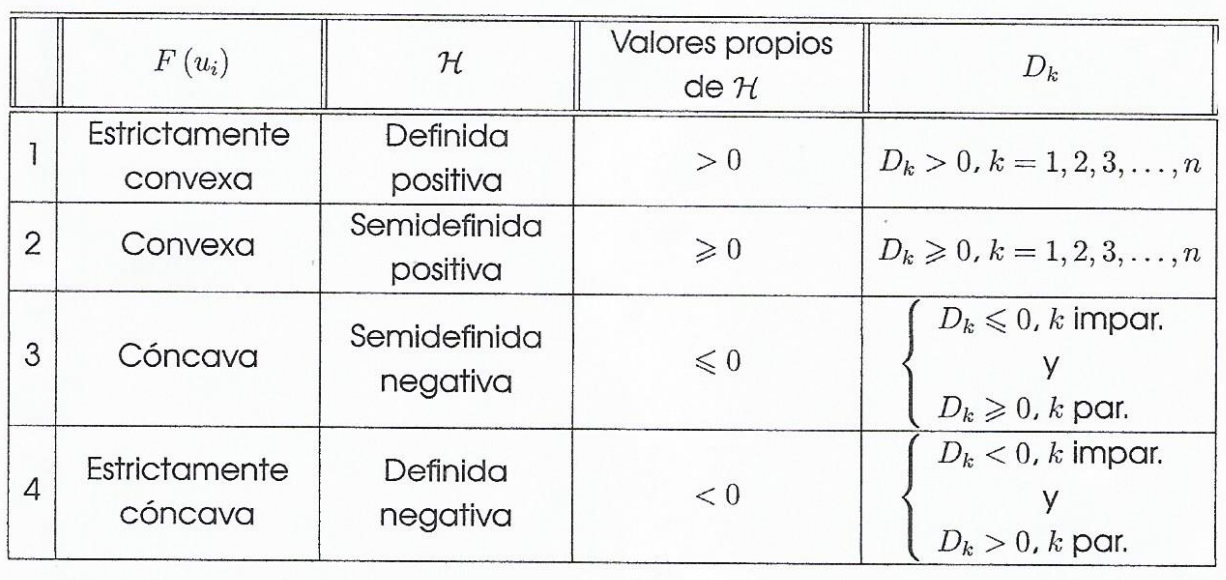
\includegraphics[scale=0.5]{figs/tabla.PNG}
\end{center}
y si la función no es convexa ni cóncava, entonces se dice que es indefinida.

\textcolor{blue}{Ejemplo:} Determinar si la función $F: \mathbb{R}^2\rightarrow \mathbb{R}$
\begin{equation*}
    F(u_1, u_2)=u^4_1+u^2_2
\end{equation*}
es concava o convexa.

\textcolor{red}{Solución:} 

Hallamas la matriz Hessiana
\begin{equation*}
    \mathcal{H}=
    \begin{pmatrix}
        \pdv{^2 F}{u^2_1} & \pdv{^2 F}{u_1 \partial u_2} \\
        \pdv{^2 F}{u_2 \partial u_1} & \pdv{^2 F}{u^2_2}
    \end{pmatrix}
    =
    \begin{pmatrix}
        12u^2_1 & 0\\
        0 & 2
    \end{pmatrix}
\end{equation*}
Hallando los menores principales 
\begin{equation*}
    D_1=12u^2_1\geq 0;\quad D_2=
    \begin{vmatrix}
        12u^2_1 & 0 \\
        0 & 2
    \end{vmatrix}
    =24u^2_1\geq 0
\end{equation*}
utilizando la tabla notamos que $F(u_1, u_2)$ es convexa.

\subsubsection{Transformada de Legendre para una v. independiente}
Dada una función $F(u)$, la transformada de Legendre proporciona una forma más conveniente de almacenar la información en la función cuando se cumple:
\begin{enumerate}
    \item La función es suave(tiene derivadas continuas).
    \item La función $F(u)$ es convexa(estrictamente).
\end{enumerate}
\begin{minipage}{0.5\textwidth}
    De la figura:
    \begin{equation}
        \tan \sigma=v=\dfrac{F+G}{u}=\dv{F(u)}{u}
    \end{equation}
    donde 
    \begin{equation}
        G(v)=uv-F(u)
    \end{equation}
    esta es la transformada de Legendre para una variable independiente. La función $G(v)$ es la transformada de Legendre de $F(u)$.
\end{minipage}
\begin{minipage}{0.5\textwidth}
    \begin{center}
        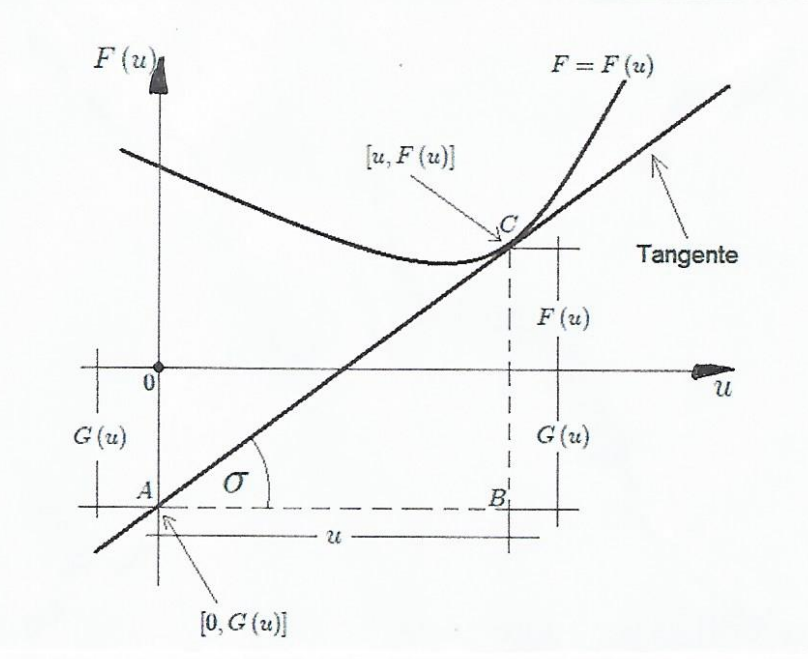
\includegraphics[scale=0.45]{figs/legendre1.PNG}
    \end{center}
\end{minipage}

\textcolor{blue}{Ejemplo:} Sea $F(u)=au^2+bu+c$, donde $a, b$ y $c$ son constantes, encontrar su transformación de Legendre 

\textcolor{red}{Solución:}

Sabemos que:
\begin{equation*}
    G(v)=uv-F(u)=uv-(au^2+bu+c)
\end{equation*}
entonces 
\begin{equation*}
    v=\dv{F(u)}{u}=2au+b \ \rightarrow \ u(v)=\dfrac{1}{2a}(v-b)
\end{equation*}
quedando así 
\begin{equation*}
    \begin{split}
        G(v)&=\dfrac{1}{2a}(v-b)v-\left[a\left(\dfrac{1}{2a}(v-b)\right)^2+b\left(\dfrac{1}{2a}(v-b)\right)+c\right]\\
        \therefore G(v)&=\dfrac{1}{4a}(v-b)^2-c    
    \end{split}
\end{equation*}

\subsubsection{Transformada de Legendre para más de una v. indep.}
Usando el desarrollo anterior para cada variable y luego generalizando
\begin{equation}
    G(v_j)=\sum_{i=1}^n u_i v_i-F(u_j);\quad j=1, \cdots, n
\end{equation}
donde $G(v_j)$ es la transformada de Legendre para $n$ variables independientes $u_j$, con 
\begin{equation}
    v_j=\pdv{F(u_i)}{u_j}
\end{equation}

\textcolor{blue}{Ejemplo:} Encuentre la transformada de Legendre $G(v_1, v_2, v_3)$ de la función: $F(u_1, u_2, u_3)=u^2_1+cu_3\sin u_2$ donde $c$ es una constante.

\textcolor{red}{Solución:}

Tenemos $n=3$ variables independientes 
\begin{equation*}
    G(v_1, v_2, v_3)=u_1v_1+u_2v_2+u_3v_3-(u^2_1+cu_3\sin u_2)
\end{equation*}
Luego 
\begin{align*}
    v_1&=\pdv{F}{u_1}=2u_1 \ \rightarrow \ u_1=\dfrac{v_1}{2}\\
    v_2&=\pdv{F}{u_2}=cu_3\cos u_2 \ \rightarrow \ u_3=\dfrac{v_2}{c}\sec u_2\\
    v_3&=\pdv{F}{u_3}=c\sin u_2 \ \rightarrow \ u_2=\sin^{-1} \left(\dfrac{v_3}{c}\right)
\end{align*}
Entonces 
\begin{equation*}
    u_3=\dfrac{v_2}{c}\sec\left[\sin^{-1}\left(\dfrac{v_3}{c}\right)\right]=\dfrac{v_2}{\sqrt{c^2-v^2_3}}
\end{equation*}
calculando $G(v_1, v_2, v_3)$
\begin{align*}
    G(v_1, v_2, v_3)&=\dfrac{v_1}{2}v_1+v_2\sin^{-1}\left(\dfrac{v_3}{c}\right)+\dfrac{v_3 v_2}{\sqrt{c^2-v^2_3}}-\left\{\left(\dfrac{v_1}{2}\right)^2+c\dfrac{\sqrt{2}}{\sqrt{c^2-v^2_3}}\sin\left[\sin^{-1}\left(\dfrac{v_3}{c}\right)\right]\right\}
\end{align*}
simplificando
\begin{equation*}
    \therefore G(v_1, v_2, v_3)=\dfrac{v^2_1}{4}+v_2\sin^{-1}\left(\dfrac{v_3}{c}\right)
\end{equation*}

\subsection{Ecuaciones canónicas de Hamilton}

Consideremos una función de dos variables $f(x, y)$
\begin{equation}
    \mathrm{d}f=\pdv{f}{x}\mathrm{d}x+\pdv{f}{y}\mathrm{d}y=u\mathrm{d}x+v\mathrm{d}y
    \left\{
    \begin{array}{c}
        \displaystyle u=\pdv{f}{x}\\ \\
        \displaystyle v=\pdv{f}{y}
    \end{array}
    \right.
\end{equation}
queremos cambiar las variables $x, y$ por las variables $u, y$ de manera que las cantidades se expresen en función de $\mathrm{d}u$ y $\mathrm{d}y$.

Sea $g=g(u, y)$ definida por 
\begin{equation}
    g=f-ux
\end{equation}
entonces: 
\begin{equation}
    \begin{split}
        \mathrm{d}g&=\mathrm{d}f-u\mathrm{d}x-x\mathrm{d}u \\
        \mathrm{d}g&=u\mathrm{d}x+v\mathrm{d}y-u\mathrm{d}x-x\mathrm{du}\\
        \mathrm{d}g=v\mathrm{d}y-x\mathrm{d}u
    \end{split}
\end{equation}
con $x=-\pdv{g}{u}$ y $v=\pdv{g}{y}$.

Aplicando esta teoría a la Hamiltoniana. Calculando $\mathrm{d}H$
\begin{equation}
    \mathrm{d}H=\sum_{i=1}^n \left(\mathrm{d}\dot{q}_i p_i+\dot{q}_i \mathrm{d}p_i\right)-\left\{\sum_{i=1}^n\left(\pdv{L}{q_i}\mathrm{d}q_i+\pdv{L}{\dot{q}_i}\mathrm{d}\dot{q}_i\right)+\pdv{L}{t}\right\}
\end{equation}
donde $\mathrm{d}\dot{q}_i p_i=0$ y $\pdv{L}{\dot{q}_i}=p_i \ \rightarrow \ \pdv{L}{\dot{q}_i}\mathrm{d}\dot{q}_i=0$. De las ecuaciones de Lagrange 
\begin{equation}
    \dv{}{t}\left(\pdv{L}{\dot{q}_i}\right)-\pdv{L}{q_i}=0 \ \rightarrow \ \dot{p}_i=\pdv{L}{q_i}
\end{equation}
por tanto 
\begin{equation}
    \mathrm{d}H=\sum_{i=1}^n (\dot{q}_i \mathrm{d}p_i-\dot{p}_i \mathrm{d}q_i)-\pdv{L}{t}\mathrm{d}t
\end{equation}
pero
\begin{equation}
    \mathrm{d}H=\sum\left(\pdv{H}{q_i}\mathrm{d}q_i+\pdv{H}{p_i}\mathrm{d}p_i\right)+\pdv{H}{t}\mathrm{d}t
\end{equation}

Las ecuaciones de Hamilton o ecuaciones canónicas de Hamilton son
\begin{equation}
    \dot{q}_i=\pdv{H}{p_i},\quad \dot{p}_i=-\pdv{H}{q_i},\quad i=1, \cdots, n
\end{equation}
también 
\begin{equation}
    \pdv{H}{t}=-\pdv{L}{t}
\end{equation}

\subsection{Formulación Lagrangiana}
\begin{minipage}{0.6\textwidth}
    El espacio de configuración no caracteriza el estado del sistema. Para caracterizar la evolución de un sistema mecánico no es suficiente con especificar la posición de las partículas sino también su velocidad de los mismos.
\end{minipage}
\begin{minipage}{0.4\textwidth}
    \begin{center}
        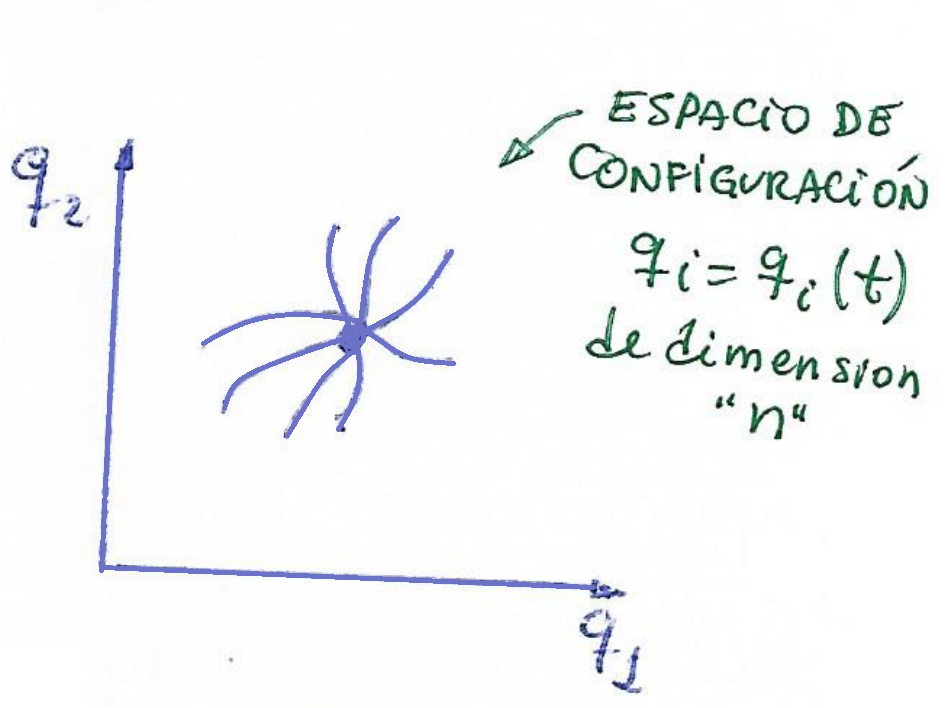
\includegraphics[scale=0.3]{figs/img3.1.PNG}
    \end{center}
\end{minipage}

\subsection{Formulación Hamiltoniana}
\begin{minipage}{0.6\textwidth}
    La formulación Hamiltoniana en lugar de espacio de configuración introduce el llamado \textbf{espacio de fase}. El espacio de fase es un espacio de dimensión $2n$ en el cual las trayectorias no se cortan. Un punto en el espacio de fase especifica completamente el estado de un estado mecánico.
\end{minipage}
\begin{minipage}{0.4\textwidth}
    \begin{center}
        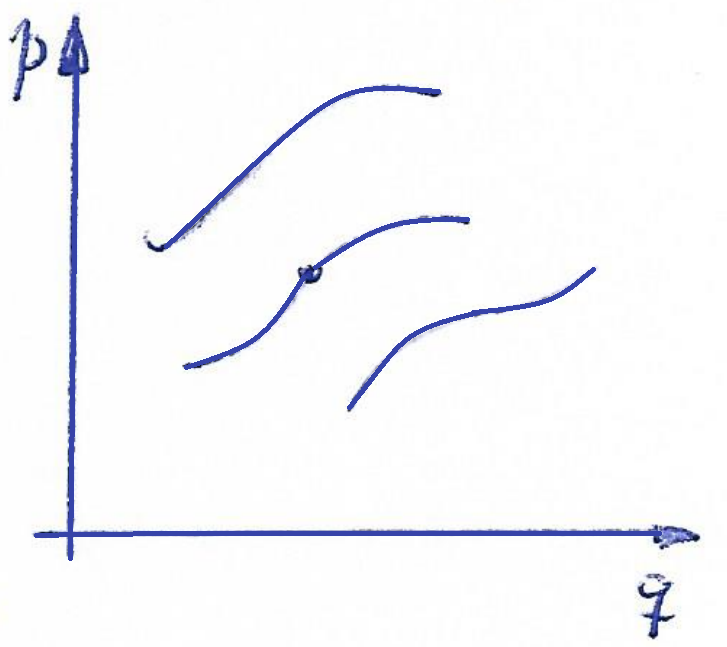
\includegraphics[scale=0.3]{figs/img3.2.PNG}
    \end{center}
\end{minipage}
Considerando que
\begin{equation}
    L=T-V
\end{equation}
donde $V$ no depende de las velocidades y $T$ es función puramente cuadrática de las velocidades.
\begin{equation}
    p_i=\pdv{L}{\dot{q}_i}=\pdv{T}{\dot{q}_i} \ \rightarrow \ H=\sum p_i \dot{q}_i-L=\sum \dot{q}_i \pdv{T}{\dot{q}_i}-(T-V)
\end{equation}

Sabemos que por el teorema de Euler de las funciones homogéneas 
\begin{equation}
    \sum \dot{q}_i \pdv{T}{\dot{q}_i}=2T
\end{equation}
Por tanto 
\begin{equation}
    \begin{split}
        H&=2T-T+V=T+V\\
        H&=E
    \end{split}
\end{equation}
la cual es la energía total del sistema.

\textcolor{blue}{Ejemplo:} Particula en un potencial central
\begin{equation*}
    L=\dfrac{m}{2}(\dot{r}^2+r^2\dot{\theta}^2+r^2\sin^2 \theta \dot{\varphi}^2)-V(r)
\end{equation*}

Sus momentos canónicos 
\begin{align*}
    p_r&=\pdv{L}{\dot{r}}=m\dot{r} \ \rightarrow \ \dot{r}=\dfrac{p_r}{m}\\
    p_{\theta}&=\pdv{L}{\dot{\theta}}=mr^2\dot{\theta} \ \rightarrow \ \dot{\theta}=\dfrac{p_{\theta}}{mr^2}\\
    p_{\varphi}&=\pdv{L}{\dot{\varphi}}=mr^2 \sin^2 \theta \ \rightarrow \ \dot{\varphi}=\dfrac{p_{\varphi}}{mr^2\sin^2 \theta}
\end{align*}
Como $H=\sum p_i \dot{q}_i-L$, entonces 
\begin{align*}
    H&=\dot{r}p_r+\dot{\theta}p_{\theta}+\dot{\varphi}p_{\varphi}-L\\
    H&=\dfrac{p_r}{m}p_r+\dfrac{p_{\theta}}{mr^2}p_{\theta}+\dfrac{p_{\varphi}}{mr^2 \sin^2\theta}p_{\varphi}-\left[\dfrac{m}{2}\dfrac{p^2_r}{m^2}+r^2\dfrac{p^2_{\theta}}{mr^4}+r^2\sin^2\theta\left(\dfrac{p_{\varphi}}{mr^2\sin^2 \theta}\right)^2-V(r)\right]\\
    H&=\dfrac{p^2_r}{2m}+\dfrac{p^2_{\theta}}{2mr^2}+\dfrac{p^2_{\varphi}}{2mr^2\sin^2\theta}+V(r)
\end{align*}

Notar que: $H=H(r, \theta, \varphi, p_r, p_{\theta}, p_{\varphi})$. Las ecuaciones de Hamilton son:
\begin{equation*}
    q_i=\pdv{H}{p_i} \rightarrow 
    \left\{
    \begin{split}
        \dot{r}&=\pdv{H}{p_r}=\dfrac{p_r}{m}\\
        \dot{\theta}&=\pdv{H}{p_{\theta}}=\dfrac{p_{\theta}}{mr^2}\\
        \dot{\varphi}&=\pdv{H}{p_{\varphi}}=\dfrac{p_{\varphi}}{mr^2\sin^2 \theta}
    \end{split}
    \right.        
\end{equation*}
\begin{equation*}
    \dot{p}_i=-\pdv{H}{q_i} \rightarrow 
        \left\{
        \begin{split}
            \dot{p}_r&=-\pdv{H}{r}=\dfrac{p^2_{\theta}}{mr^3}+\dfrac{p^2_{\varphi}}{mr^3 \sin^2 \theta}-\dv{V}{r}\\
            \dot{p}_{\theta}&=-\pdv{H}{\theta}=\dfrac{p^2_{\varphi} \cot \theta}{mr^2\sin^2 \theta}\\
            \dot{p}_{\varphi}&=-\pdv{H}{\varphi}=0
        \end{split}
        \right.
\end{equation*}

\textit{Teorema:} Si $H$ no depende explicitamente del tiempo, entonces $H$ es constante de movimiento.

\textcolor{red}{Demostración:} Como $H=H(q, p, t)$
\begin{equation}
    \dv{H}{t}=\sum_{i=1}^n\left(\pdv{}{q_i}\dot{q}_i+\pdv{H}{p_i}\dot{p}_i\right)+\pdv{H}{t}
\end{equation}
usando las ecuaciones de Hamilton 
\begin{equation}
    \dv{H}{t}=\sum_i \underbrace{\left(\pdv{H}{q_i}\pdv{H}{p_i}-\pdv{H}{p_i}\pdv{H}{q_i}\right)}_{0}+\pdv{H}{t}=\pdv{H}{t}
\end{equation}
Si $\pdv{H}{t}=0$, entonces
\begin{equation}
    \therefore \dv{H}{t}=0 \ \rightarrow \ H=\text{cte}
\end{equation}

Pueden suceder las siguientes condiciones 
\begin{enumerate}
    \item[$i$)] $H=\text{cte}$ pero $H\neq E$.
    \item[$ii$)] $H=E$ pero $H\neq \text{cte}$. 
\end{enumerate}

\textcolor{blue}{Ejemplo:} Considere una esferita de masa $m$ que puede deslizarse, sin rozamiento, por un alambre que gira en un plano horizontal 

\textcolor{red}{Solución:}

El lagrangiano 
\begin{equation}
    L=T=\dfrac{m}{2}(\dot{r}^2+r^2\dot{\theta}^2)
\end{equation}

La hamiltoniana 
\begin{equation}
    p_r=\pdv{L}{\dot{r}}=m\dot{r}
\end{equation}
entonces 
\begin{equation}
    \begin{split}
        H&=\dot{r}p_r-L=\dfrac{p_r}{m}p_r-\dfrac{m}{2}\left(\dfrac{p^2_r}{m^2}+\omega^2 r^2\right)\\
        H&=\dfrac{p^2_r}{2m}-\dfrac{m\omega^2}{2}r^2
    \end{split}
\end{equation}
así 
\begin{align*}
    i&) \pdv{H}{t}=0 \ \rightarrow \ H=\text{cte}\\
    ii&) H\neq E=T
\end{align*}

\section*{Problemas}
\begin{enumerate}
    \item Dada la Lagrangiana 
    \begin{equation}
        L=\dfrac{m\dot{q}^2}{2}-\dfrac{1}{2}kq^2+\lambda \dot{q}q
    \end{equation}
    \begin{enumerate}[label=(\alph*)]
        \item Hallar la Hamiltoniana.
        \item Hallar las ecuaciones de Hamilton.
    \end{enumerate}
    \item Una partícula de masa $m$ se mueve bajo la influencia de la gravedad a lo largo de la espiral $z=k\varphi$, como se muestra en la figura, donde $r$ y $k$ son constantes. Hallar las ecuaciones de movimiento de Hamilton.
    \item Una particula de masa $m$ se mueve en una dimensión bajo la influencia de la fuerza 
    \begin{equation}
        F(x, t)=\dfrac{k}{x^2}e^{-t/\tau}
    \end{equation}
    donde $k$ y $\tau$ son constantes.
    \begin{enumerate}[label=(\alph*)]
        \item Encuentre la función de Hamilton o Hamiltoniana.
        \item Halle las ecuaciones de Hamilton.
        \item ¿Es la Hamiltoniana igual a la energía total?
    \end{enumerate}
    \item Obtenga el Hamiltoniano y las ecuaciones de movimiento de una partícula de masa $m$ que desliza sin rozamiento por el interior de un casquete de radio $R$ de forma esférica. ¿Qué constantes de movimiento posee el sistema?
\end{enumerate}

\section*{Problemas Final}
\begin{enumerate}
    \item La figura muestra una cuenta(una pequeña esfera con un orificio central) de masa $m$ que puede moverse libremente a lo largo de un aro de radio $R$ y masa despreciable. El aro, a su vez, gira con frecuencia angular $w$ constante alrededor del eje vertical $z$. Sea $\theta$ el ángulo que el vector posición de la cuenta hace con la dirección vertical. La aceleración de la gravedad se denota por $\vec{g}$.
    \begin{enumerate}[label=(\alph*)]
        \item Calcula la lagrangiana $L(\theta, \dot{\theta})$ de la partícula.
        \item Demuestre que la hamiltoniana puede ser escrita en la forma 
        \begin{equation*}
            H(\theta, p)=\dfrac{p^2}{2mR^2}-\dfrac{mR^2 w^2 \sin^2 \theta}{2}-mgR \cos \theta
        \end{equation*}
        \item Partiendo de las ecuaciones de Hamilton, obtenga las ecuaciones de movimiento del sistema.
        \item Si $p$ es constante, demuestre que $\theta=\arccos (g/Rw^2)$.
        \item ¿Es posible afirmar que la hamiltoniana del item (b) corresponde a la energía total del sistema? Justifique su respuesta.
    \end{enumerate}
    \item 
    \begin{enumerate}[label=(\alph*)]
        \item Encuentre la transformación canónica generada por
        \begin{equation*}
            F(q, Q)=\lambda q^2 \cot Q,
        \end{equation*}
        donde $\lambda$ es una constante.
        \item Si en la representación $(Q, P)$ la hamiltoniana es 
        \begin{equation*}
            K(Q, P)=\left(\dfrac{2\lambda}{\mu}\cos^2 Q+\dfrac{\mu\Omega^2}{2\Lambda}\sin^2 Q\right)P,
        \end{equation*}
        donde $\mu$ y $\Omega$ son constantes, encuentre la hamiltoniana $H(q, p)$ en l representación $(q, p)$.
        \item Encuentre el valor de $\lambda$ tal que $K(Q, P)$ sea independiente de $Q$ y describa el movimiento en las representaciones $(Q, P)$ y $(q, p)$.
    \end{enumerate}
    \item Considere un movimiento unidimensional de una partícula con coordenadas generalizadas $q$, cuya lagrangiana es dada por 
    \begin{equation*}
        L(q, \dot{q})=\dfrac{1}{2}\left(\dfrac{\dot{q}^2}{q^4}-\dfrac{1}{q^2}\right)
    \end{equation*}
    \begin{enumerate}[label=(\alph*)]
        \item Obtenga la hamiltoniana del sistema $H(q, p)$ en términos de la coordenada $q$ y $p$.
        \item Utilizando la función generadora de primer tipo $F(q, Q)=-Q/q$, obtenga la transformación $Q=pq^2$ y $P=1/q$, donde $Q$ y $P$ representan respectivamente las coordenadas y el momento transformados. Verifique que esa transformación es canónica.
        \item Calcule la hamiltoniana transformada $K=K(Q, P)$ y resuelva las ecuaciones de Hamilton de movimiento para la coordenada $Q=Q(t)$ y momento $P=P(t)$ considere las siguientes condiciones iniciales $Q(0)=1$ y $P(0)=0$.
        \item De los resultados anteriores calcule la expresión para $q=q(t)$ y $p=p(t)$. Verifique explicitamente que esta solución satisface la ecuación de Hamilton para $H(q, p)$.
    \end{enumerate}
    \item Considere una partícula descrita por la hamiltoniana
    \begin{equation*}
        H=\dfrac{p^2}{2m}-kxe^{-\lambda t}
    \end{equation*}
    donde $m$ es la masa, $k$ y $\lambda$ son constantes positivas.
    \begin{enumerate}[label=(\alph*)]
        \item Resuelva la ecuación de Hamilton-Jacobi 
        \begin{equation*}
            \pdv{S}{t}+H(x, p=\pdv{S}{q}, t)=0.
        \end{equation*}
        \item Obtenga la posición $x(t)$ y el momento lineal $p(t)$ de la partícula para las condiciones iniciales $x(0)=0=p(0)$.
        \item Calcule la aceleración $a(t)$ y describa el movimiento de la partícula para $t>0$ y $t>>1/t$.
    \end{enumerate}
    \item Se tiene un proyectil (partícula puntual de masa $m$) que es disparado en un tiempo $t=0$ desde el origen de coordenadas con una velocidad inicial $v_0$ y un ángulo $\alpha$ con la horizontal, en presencia de un campo de fuerzas gravitatorio. Considerando el movimiento en dos dimensiones(plano $xy$), calcular lo siguiente utilizando el formalismo de Hamilton-Jacobi. Considere que la aceleración de la gravedad, de magnitud $g$ esta en al dirección $y$ y que en la dirección $x$ actua una aceleración $a_x=g/2$. Hallar
    \begin{enumerate}[label=(\alph*)]
        \item Las ecuaciones de movimiento para cada coordenada: $y(t)$ y $x(t)$.
        \item La ecuación de la trayectoria, $y(x)$.
    \end{enumerate}
    Utilizar las condiciones iniciales para obtener el valor de las constantes obtenidas por el método.
\end{enumerate}
\end{document}